\documentclass[11pt,letterpaper]{article}
\usepackage{float}
\usepackage[top=0.85in,left=1.75in,footskip=0.75in,marginparwidth=2in]{geometry}

\raggedright
\setlength{\parindent}{0.5cm}
\textwidth 5.5in 
\textheight 8.75in

% use Unicode characters - try changing the option if you run into troubles with special characters (e.g. umlauts)
\usepackage[utf8]{inputenc}

% line numbers
\usepackage{lineno}

% clean citations
% miles: use natbib instead of whatever default is in biorxiv template
\usepackage{natbib}

% improves typesetting in LaTeX
\usepackage{microtype}
\DisableLigatures[f]{encoding = *, family = * }

% use adjustwidth environment to exceed text width (see examples in text)
\usepackage{changepage}

% adjust caption style
\usepackage[aboveskip=1pt,labelfont=bf,labelsep=period,singlelinecheck=off]{caption}

\usepackage{booktabs}
\usepackage{array}
\usepackage{multirow}
\usepackage{amsmath}
\usepackage{amssymb}
\usepackage{graphicx}
\usepackage{gensymb}
\usepackage{epstopdf}

%text color
\usepackage{xcolor}

% hyperref makes references clicky. use \url{www.example.com} or \href{www.example.com}{description} to add a clicky url
\usepackage{nameref,hyperref}
\hypersetup{
    colorlinks=true,
    linkcolor=blue,
    citecolor=black,      
    urlcolor=blue,
}

\usepackage[colorinlistoftodos]{todonotes}
\newcommand{\emjo}[1]{\todo[size=\scriptsize, color=purple!50]{#1}}
\newcommand{\jeremy}[1]{\todo[size=\scriptsize, color=green!50]{#1}}
\newcommand{\dothis}[1]{\textcolor{purple}{\textbf{#1}}}



\newcommand{\beginsupplement}{%
        \setcounter{table}{0}
        \renewcommand{\thetable}{S\arabic{table}}%
        \setcounter{figure}{0}
        \renewcommand{\thefigure}{S\arabic{figure}}%
}

\newcommand{\gxe}{$G \times E$}
\newcommand{\qpc}{$Q_{PC}$}
\newcommand{\qf}{$Q_{ST}-F_{ST}$}

% title goes here:
\begin{document}
\begin{flushleft}
\textbf\newline
{\Large
\textbf\newline{Multivariate adaptive divergence contributes to $G \times E$ in \textit{Arabidopsis thaliana}}
}
\newline


% authors go here:

Emily B. Josephs \textsuperscript{1,2,3},
Husain I. Agha \textsuperscript{1,2,3}, \&
Jeremy J. Berg \textsuperscript{4}
\\
\bigskip
\bf{1} Department of Plant Biology, Michigan State University, East Lansing, MI
\\
\bf{2} Ecology, Evolution, and Behavior Program, Michigan State University, East Lansing, MI
\\
\bf{3} Plant Resilience Institute, Michigan State University, East Lansing, MI
\\
\bf{4} Department of Human Genetics, University of Chicago, Chicago, IL
\\
\bigskip
* josep993@msu.edu
\end{flushleft}
\bibliographystyle{newphyt}

\linenumbers

\section*{Abstract}
Determining the evolutionary forces shaping genetic variation for environmental responses (\gxe) is crucial for comprehensively understanding local adaptation and predicting responses to new environments. 
We expect local adaptation for environmental responses to contribute to \gxe\ on a species-wide scale but we lack evidence of this process, in part because we lack rigorous methods for detecting it.
One challenge in developing these methods is that the different ways that \gxe\ has been conceptualized, as reaction norms and as correlated traits, can lead to different interpretations.
Here we apply methods based on \qf\ to a large multi-environment datasets from \textit{Arabidopsis thaliana}.
\textcolor{purple}{Summary of results}
For flowering time measured in outdoor common gardens, we do detect evidence of local adaptation for environmental responses to season.
Overall, these results suggest that local adaptation does contribute to \gxe\ in \textit{A. thaliana} and that these methods could be broadly applied to comprehensively evaluate the role of local adaptation in shaping \gxe.

\section*{Introduction}

%Big picture
Traits are shaped by both genetics and the environment, so determining the evolutionary forces shaping trait variation requires not only identifying genetic variation for traits but also determining how this variation differs across environments.
Genetic variation for environmental response (or plasticity) can contribute to genotype by environment interactions (\gxe) in determining phenotypes \citep{falconer1952problem, bradshaw1965evolutionary}.
\gxe\ has long been of interest to evolutionary biologists because it could represent adaptive phenotypic plasticity  \citep{schlichting1986evolution,scheiner1993genetics}.
While adaptation through the evolution of plastic responses could increase fitness in heterogeneous environments \citep{van1991evolution, baythavong2011linking, anderson2021selection}, the evolution of plasticity could be limited by costs or other factors \citep{dewitt1998costs, callahan2005plasticity, roberts2023weaker}.
Alternatively, \gxe\ could result from different selection pressures across environments that constrain trait expression in some environments but allow trait expression to drift in environments where selection is relaxed \citep{paaby2014cryptic}.
Distinguishing between these scenarios has been challenging.

Different conceptions of plasticity have contributed to different methods for investigating the evolutionary forces shaping \gxe.
First, plasticity could be measured using reaction norms: functions of trait value expression across environments \citep{freeman1973statistical,scheiner1993genetics, morrissey2016variation, arnold2019analyse, de2025partitioning}.
Reaction norms have been studied in a number of contexts and been used to test for selection on plasticity \citep{valdes2023spring, wagner2018plasticity}.
One limitation of reaction norms is often they require doing 'statistics on statistics', losing variance when estimating reaction norms, although the random regression approach alleviates this issue \citep{arnold2019analyse}.
Second, trait values measured across environments can be thought of as correlated traits, and methods developed for studying multivariate trait evolution can be applied to plasticity.
Studies of plasticity as a multivariate trait have found that the genetic basis of traits differs across environments \citep{yan2021genetic}, identified specific types of weather contributing to phenological \gxe\ \citep{MacQueen_2025}, and measured selection for plasticity\citep {anderson2021selection}.

Alongside different ways of measuring plasticity, a number of experimental approaches have been used to test whether local adaptation for plasticity contributes to \gxe.
First, common garden experiments in different natural environments or in manipulated environmental conditions have looked for evidence of associations between fitness and plasticity \citep{stinchcombe2004flowering, scheiner1999measuring, dudley1996testing, baythavong2010characterizing}.
However, these types of manipulative experiments are not possible without either a plastic response that can be permanently induced, like shade response, or enough genetic variation in plasticity to detect a relationship between plasticity and fitness.
They are also limited to detecting selection acting on plasticity in the specific experimental year, but multi-year experiments have found significant temporal variation \citep{oakley2023ecological}.


In contrast, \qf\ and related methods test for local adaptation by determining whether among-population trait divergence exceeds expectations under drift \citep{prout1993f, spitze1993population, whitlock2008evolutionary, ovaskainen2011new, karhunen2013driftsel}.
The few previous applications of \qf\ to reaction norms have not detected evidence of adaptive divergence \citep{von2008partitioning,de2016evolution,lind2011gene} and these approaches have not been applied to the correlated trait way of measuring plasticity, although approaches exist for using \qf\ to detect selection on correlated traits \citep{chenoweth2008q, kremer1997multilocus}.
Additional studies have compared $Q_{ST}$ values across environments as an indirect way of investigating selection on plasticity \citep{ramirez2018natural, rodriguez2016capturing, hangartner2012adaptive, palo2003latitudinal}. 
Inferences from \qf\ can be inaccurate when population relatedness does not match a simple island model \citep{de2022common}.
Recent extensions of \qf\ have made it possible to use these inferences on more complicated diversity panels \citep{do2025method, ovaskainen2011new} and on structured diversity panels that are common in genome-wide association mapping studies \citep{Josephs2019}.
However, we lack clear methods and approaches for using \qf\ approaches to investigate plasticity, for either a reaction norm or correlated trait approach.


Life history timing is a crucial aspect of fitness and the ideal timing of life history events depends on the environment \citep{worthy2025accelerated, aagren2017adaptive, colautti2013rapid}.
Flowering time in the plant species \textit{Arabidopsis thaliana} is a classic model for studying the evolution of plasticity and \gxe\  \citep{mitchell2006genetic, maple2024flowering, leventhal2025planting}.
As would be expected for an annual plant with a large geographic range, \textit{A. thaliana} ecotypes exhibit a range of life history strategies and these strategies can often be connected to environmental or geographic variation, contributing to \gxe\ \citep{stinchcombe2004latitudinal, mitchell2006genetic, hancock2011adaptation,martinez2020functional}.
%In addition, many QTLs for flowering time are environment specific \citep{li2014genetic, li2010association}.
Vernalization, the cold temperatures experienced by overwintering plants, is an important cue for flowering time and \textit{A. thaliana} ecotypes differ in their sensitivity to vernalization \citep{shindo2006variation, sung2005remembering}.
%There is evidence for selection on one of the genes important for vernalization response, FRIGIDA \citep{Toomajian2006nonparametric}, however FRIGIDA variation alone cannot explain observed variation in response to vernalization \citep{wilczek2010genetic}.
Despite the extensive study of this trait, we lack a clear link between flowering time plasticity variation and long-term selection, limiting our understanding of how local adaptation has shaped variation in this system.

In this study, we develop methods to test for the contribution of local adaptation to \gxe.
\textcolor{purple}{summary goes here}

\section*{Materials and Methods}

\subsection*{Testing for selection on plasticity}
\cite{Josephs2019} previously developed methods for detecting selection on quantitative traits by extending $Q_{ST}-F_{ST}$ analyses to test for excess differentiation along specific principle components (PC) of genetic relatedness. 
Specifically, if $\vec{Z}$ is a mean-centered vector of trait values measured in the same environment, we can model the neutral expectation for $\vec{Z}$ as 
\begin{equation} \label{eq:mvn}
\vec{Z} \sim MVN (\vec{0}, 2V_{A}F)
\end{equation}
where $V_{A}$ is additive genetic variation and $F$ is the genetic kinship matrix for the individuals in $\vec{Z}$.

We can also model projections of the trait values onto specific genetic principal components (the eigenvectors of $F$), so that if $U_{m}$ and $\lambda_{m}$ are the $m^{th}$ eigenvector and eigenvalue of $F$,
\begin{equation}
\frac{\vec{Z}\cdot \vec{U_{m}}}{\sqrt{\lambda_{m}}} \sim N(0, 2V_{A}).
\end{equation}

Crucially, the variance of these projections onto a set of eigenvectors can be used to estimate $V_{A}$ such that 
\begin{equation}\label{eq:vaest}
V_{A, est} = \frac{1}{2\lvert \mathbb{L} \rvert} \sum_{i\in \mathbb{L}}\textnormal{Var}(\frac{\vec{Z}\cdot \vec{U_{i}}}{\sqrt{\lambda_{i}}}),
\end{equation}

where $\mathbb{L}$ is some set of principal components that does not include $m$.
Then, we can use a test statistic called $Q_{PC}$ to test for selection on a specific PC, $m$, that is not in the set used to estimate $V_{A}$. 

\begin{equation}\label{eq:qpcbasic}
Q_{PC} = \frac{\vec{Z}\cdot\vec{U_{m}}}{\sqrt{2\lambda_{m}V_{A,est}}}\sim N(0,1).
  \end{equation}

We can apply the test described in Eq. \ref{eq:qpcbasic} to any quantitative trait and also, to any additive combination of quantitative traits, like a linear reaction norm (see the supplementary material for an explanation of why this test cannot be applied to non-additive measures of plasticity).

We also expand upon a conditional test for adaptive differentiation developed by \cite{Berg2017} based on the framework of \cite{lande1979quantitative} that tests for adaptation in a given trait ('trait1') conditional on a second trait ('trait2').

\begin{equation}
Q_{PC, 1|2} = \frac{(\vec{Z_{1}} - \vec{\mu_{1}'})\vec{U_{m}}}{\sqrt{2\lambda_{m}V_{A,1}'}}  \sim N(0,1)
  \end{equation}

In contrast to the test described in Eq. \ref{eq:qpcbasic}, a conditional mean ($\vec{\mu_{1}'}$) and variance ($V_{A,1}'$) for trait1 incorporate information about trait values and additive genetic variance for trait2, along with the additive genetic covariance between traits 1 and 2.
See the supplemental material for equations calculating the conditional mean and variance.

\subsection*{Simulations}
%We conducted simulations of neutrally evolving phenotypes to evaluate the behavior of our conditional test for selection.
%We simulated two correlated traits evolving 100 individuals from the \textit{A. thaliana} population sample using the matrix.normal function from the MBSP package in R \citep{mbsp,r}.
%For these simulations, $V_{A,1} = V_{A,2} = 1$ and $C_{A,12} = 0.8$.\emjo{note that I could try extra sims varying these}
%\dothis{really need more details}

%We next simulated selection on trait2 along PC 2 of the kinship matrix by adding a selected effect equivalent to the line's position on PC 2 multiplied by $\lambda_{2}$ to each simulated value for trait2.
%We simulated the correlated effects of selection on trait1 by adding a selective effect to trait1 values equivalent to position on PC 2 multiplied by $C_{A, 12} \times \lambda_{2}$.

We used SLiM \citep{haller2025slim} to generate forward-in-time simulations of the evolution of a trait with plasticity. These Wright-Fisher simulations consisted of 100 demes with 50 individuals per deme organized in a 10 x 10 grid with a migration rate of 5\% between adjacent populations. 

%We simulated the evolution of a trait with plasticity under Gaussian stabilizing selection. 
Trait plasticity was modeled as two character states (e.g., pleiotropic traits whose expression depends on the environment) which we will refer to as trait1 and trait2. We draw the effects of a quantitative trait nucleotide (QTN) on trait1 and trait2 ($a_1$ and $a_2$) as random variables drawn from a multivariate normal distribution,

\begin{equation}
    \begin{pmatrix} a_1 \\ a_2 \end{pmatrix} \sim N\left(\begin{pmatrix} 0 \\ 0 \end{pmatrix}, \Sigma\right)
\end{equation}

where,
\begin{equation}
\Sigma = \sigma^2 \begin{pmatrix} 1 & \rho \\ \rho & 1 \end{pmatrix}
\end{equation}

$\sigma$ is 0.1 and $\rho$ is the correlation of QTN effects between traits.

The simulated populations were subject to environmentally-dependent, spatially heterogeneous, stabilizing selection. 
The optimal trait value varied along the y-axis but was constant along the x-axis, representing a clinal trait optimum across latitude.
For each generation, we modeled the effect of the individuals experiencing environment 1 or environment 2, and thus eliciting trait1 or trait2, by setting one trait to be under stabilizing selection while the other had no affect on fitness. 
Fitness was determined by the difference in an individual's expressed trait value and the optimum at that latitude by a Gaussian function

\begin{equation}
    \omega_{ijy} = \exp\{-\frac{1}{2}(\frac{T_{ijy} - \Theta_{jy}}{\sigma_\omega})^2\}
\end{equation}

where $T_{ijy}$ is the vector of $j$ character state trait values for individual $i$ in latitude $y$, $\Theta_{jy}$ is the optimum trait value for that latitude and character state, and $\sigma_\omega$ determines the strength of selection (a lower number being stronger selection).

The genome consisted of 10 independently segregating 1 Mb chromosomes with a recombination rate of $1\times10^{-7}$. 
The mutation rate for quantitative trait nucleotides (QTN) was set to $1\times10^{-8}$. 
We implemented tree sequence recording in SLiM and overlaid neutral mutations in msprime \citep{msprime} at a rate of $1\times10^{-7}$. To reduce computational load, the genome size was reduced by a factor of 10 and the recombination and mutation rates were all increased by a factor of 10 (scaled values: chromosome length 100 kb; recombination rate $1\times10^{-6}$; QTN mutation rate $1\times10^{-7}$; neutral mutation rate $1\times10^{-6}$).

For the burn-in, we simulated a single, randomly mating population with 1000 individuals and an optimal trait value of 0.0 for both character states and allowed the population to equilibrate for 10000 generations. The initial population was then used as founders for 100 demes with 50 individuals each in a 10 x 10 grid and a migration rate of 0.05 between adjacent demes. The final optimal trait values for the simulations ranged from $-1.0$ to $1.0$ and $1.0$ to $-1.0$ for for trait1 and trait2, respectively (Fig. \ref{fig:simOptima}). After the initial burn-in, the optimal trait values moved from $0.0$ to their final values over 5000 generations in a stepwise fashion. The optimal reaction norm was the difference between the trait1 and trait2 optima within each latitude (ranging from $-2.0$ to $2.0$). The simulations were run for another 10000 generations, after which final genotypes (as tree sequences) and trait values for both character states were recorded for four randomly sampled individuals per deme.

We simulated populations with varying strengths of selection ($\sigma_\omega$ = 0.5, 1.0) and correlations of QTN effects between condition states ($\rho$ = 0.6, 0.75, 0.9). We simulated trait2 evolving neutrally and under selection by setting its probability to be expressed to 0 and 0.5, respectively. We conducted 100 replicates for each combination of parameters and tested for selection on both condition states and the reaction norm (difference between trait1 and trait2) using standard and conditional $Q_{PC}$.

\subsection*{\textit{A. thaliana} data}
We evaluated our tests of selection on two datasets of \textit{A. thaliana} flowering time.
The first dataset contained data on flowering time measured in two growth chambers (16 \degree C and 10 \degree C with 16 hours of light) for 971 accessions \citep{alonso20161}.
Flowering time was measured as days to first open flower for four replicates.

The second dataset contained phenological data measured in a set of common garden experiments conducted in Norwich England \citep{fournier2011map, wilczek2009effects}. 
Seeds from 140 individuals were planting in 14 replicated blocks the same location in the fall  and in the spring and days to bolting was measured.
Fall plants were sown between September 3-7, 2006 and transplanted to the field between September 17-21 2006.
Spring plants were sown between February 25-27 2007 and transplanted between March 11-14 2007.
All sowing and transplanting was done in a random order and plants were grown in a randomized block design.
To compare these two environments, we used photothermal units to bolting instead of days to bolting.

A SNP matrix for all the accessions analyzed was downloaded from the 1001 genomes website (\url{http://1001genomes.org/data/GMI-MPI/releases/v3.1/SNP_matrix_imputed_hdf5/}, \cite{alonso20161}). 
We constructed kinship matrices for the individuals in each dataset using 50,000 randomly sampled SNPs.
In all tests of selection, we used the last half of the PCs to estimate $V_{A,1}$, $V_{A,2}$, and $C_{A,12}$.

We identified genotypes with combinations of flowering time across environments that fell outside the bounds described by the G matrix.
Our reasoning was that these genotypes have plastic responses that are distinct from most other genotypes in the sample and may provide interesting candidates for future studies.
We used the phenotypes to estimate parameters of the $2\times 2$ G matrix. Each entry in the matrix, $G_{i,j} = (\vec{Z_i} \times \vec{Z_j})/n$, where $\vec{Z_i}$ is the mean-centered vector of values for trait i (or trait j in the case of $\vec{Z_h}$ and $n$ is the number of genotypes. 
Note that these values of the matrix correspond to genetic variances where if $i=j$, $G_{i,j}$ is the genetic variance of the trait and if $i \neq j$, $G_{i,j}$ is the genetic covariance between traits.

Once the $G$ was estimated, we could use it to generate an ellipse of expected values for two traits given the values of G. 
We roughly followed the procedure used to generate figure 4 in \cite{machado2023rules}.
We plotted each genotype with the trait in environment 1 on the X axis and the trait in environment 2 on the Y axis.
We then plotted an ellipse of points corresponding to the joint $\chi ^2$ distribution of the two phenotypes at $\alpha = 0.05$


\section*{Results}

%\subsection*{Simulations of $Q_{PC}$ on reaction norms}

\subsection*{Simulations of conditional $Q_{PC}$ to detect selection on plasticity}

First, we wanted to understand how standard \qpc\ and conditional \qpc\ performed when only one character state is under selection (i.e., no selection on phenotypic plasticity). 
To do this, we conducted a total of 600 simulations where trait1 was under selection while trait2 was neutral but genetically correlated to trait1 (Fig. \ref{fig:pvalBoxplot}A, C). When trait1 was under selection but trait2 evolved neutrally, $Q_{PC}$ correctly detected selection on trait1 in all 600 simulations. The conditional test performed comparably, dropping only when the correlation of allelic effects between traits was high and selection was weak ($\rho=0.9$, $\sigma_\omega=1.0$: 0.06 false negative rate). \qpc\ on trait2, however, produced a substantial false positive rate that rose sharply with $\rho$: from 0.36 when $\rho=0.6$ to 1.0 when $\rho=0.9$ (mean: 0.738). The conditional test on trait2 resolved most of those false positives with an average false positive rate of just 0.01, well below our 0.05 significance threshold.

We then tested the performance of \qpc\ and the conditional test when both character states were under selection (i.e., selection for phenotypic plasticity; Fig. \ref{fig:pvalBoxplot}B, D). When both trait1 and trait2 were under selection, standard and conditional \qpc\ correctly detected selection on both trait1 and trait2 under every combination of $\rho$ and $\sigma_\omega$ tested. Interestingly, $p$ values were markedly smaller for the conditional test compared to standard \qpc\ and decreased with increasing values of $\rho$. This seemingly unintuitive finding was the result of a mismatch between the direction of selection for trait1 and trait2 but positive values of $\rho$. When we use the same simulation framework but $\rho$ is negative (i.e., the direction of selection and genetic correlations move trait values in the same direction), we find an increasing number of false negatives as $\rho$ approaches $-1$ with the conditional test (Fig. \ref{fig:negative_rho}), matching our expectation that conditional \qpc\ is a conservative test in cases where genetic correlations alone may be underlying apparent signals of selection.

Together, these results show that the conditional test distinguished true selection on a focal trait from spurious signal driven by a genetically correlated trait in our simulations. From a phenotypic plasticity perspective, this implies that conditional \qpc\ can be used to identify independent selection on trait expression within environment using common garden or reciprocal transplant experiments.

\begin{figure}[htbp]
  \centering
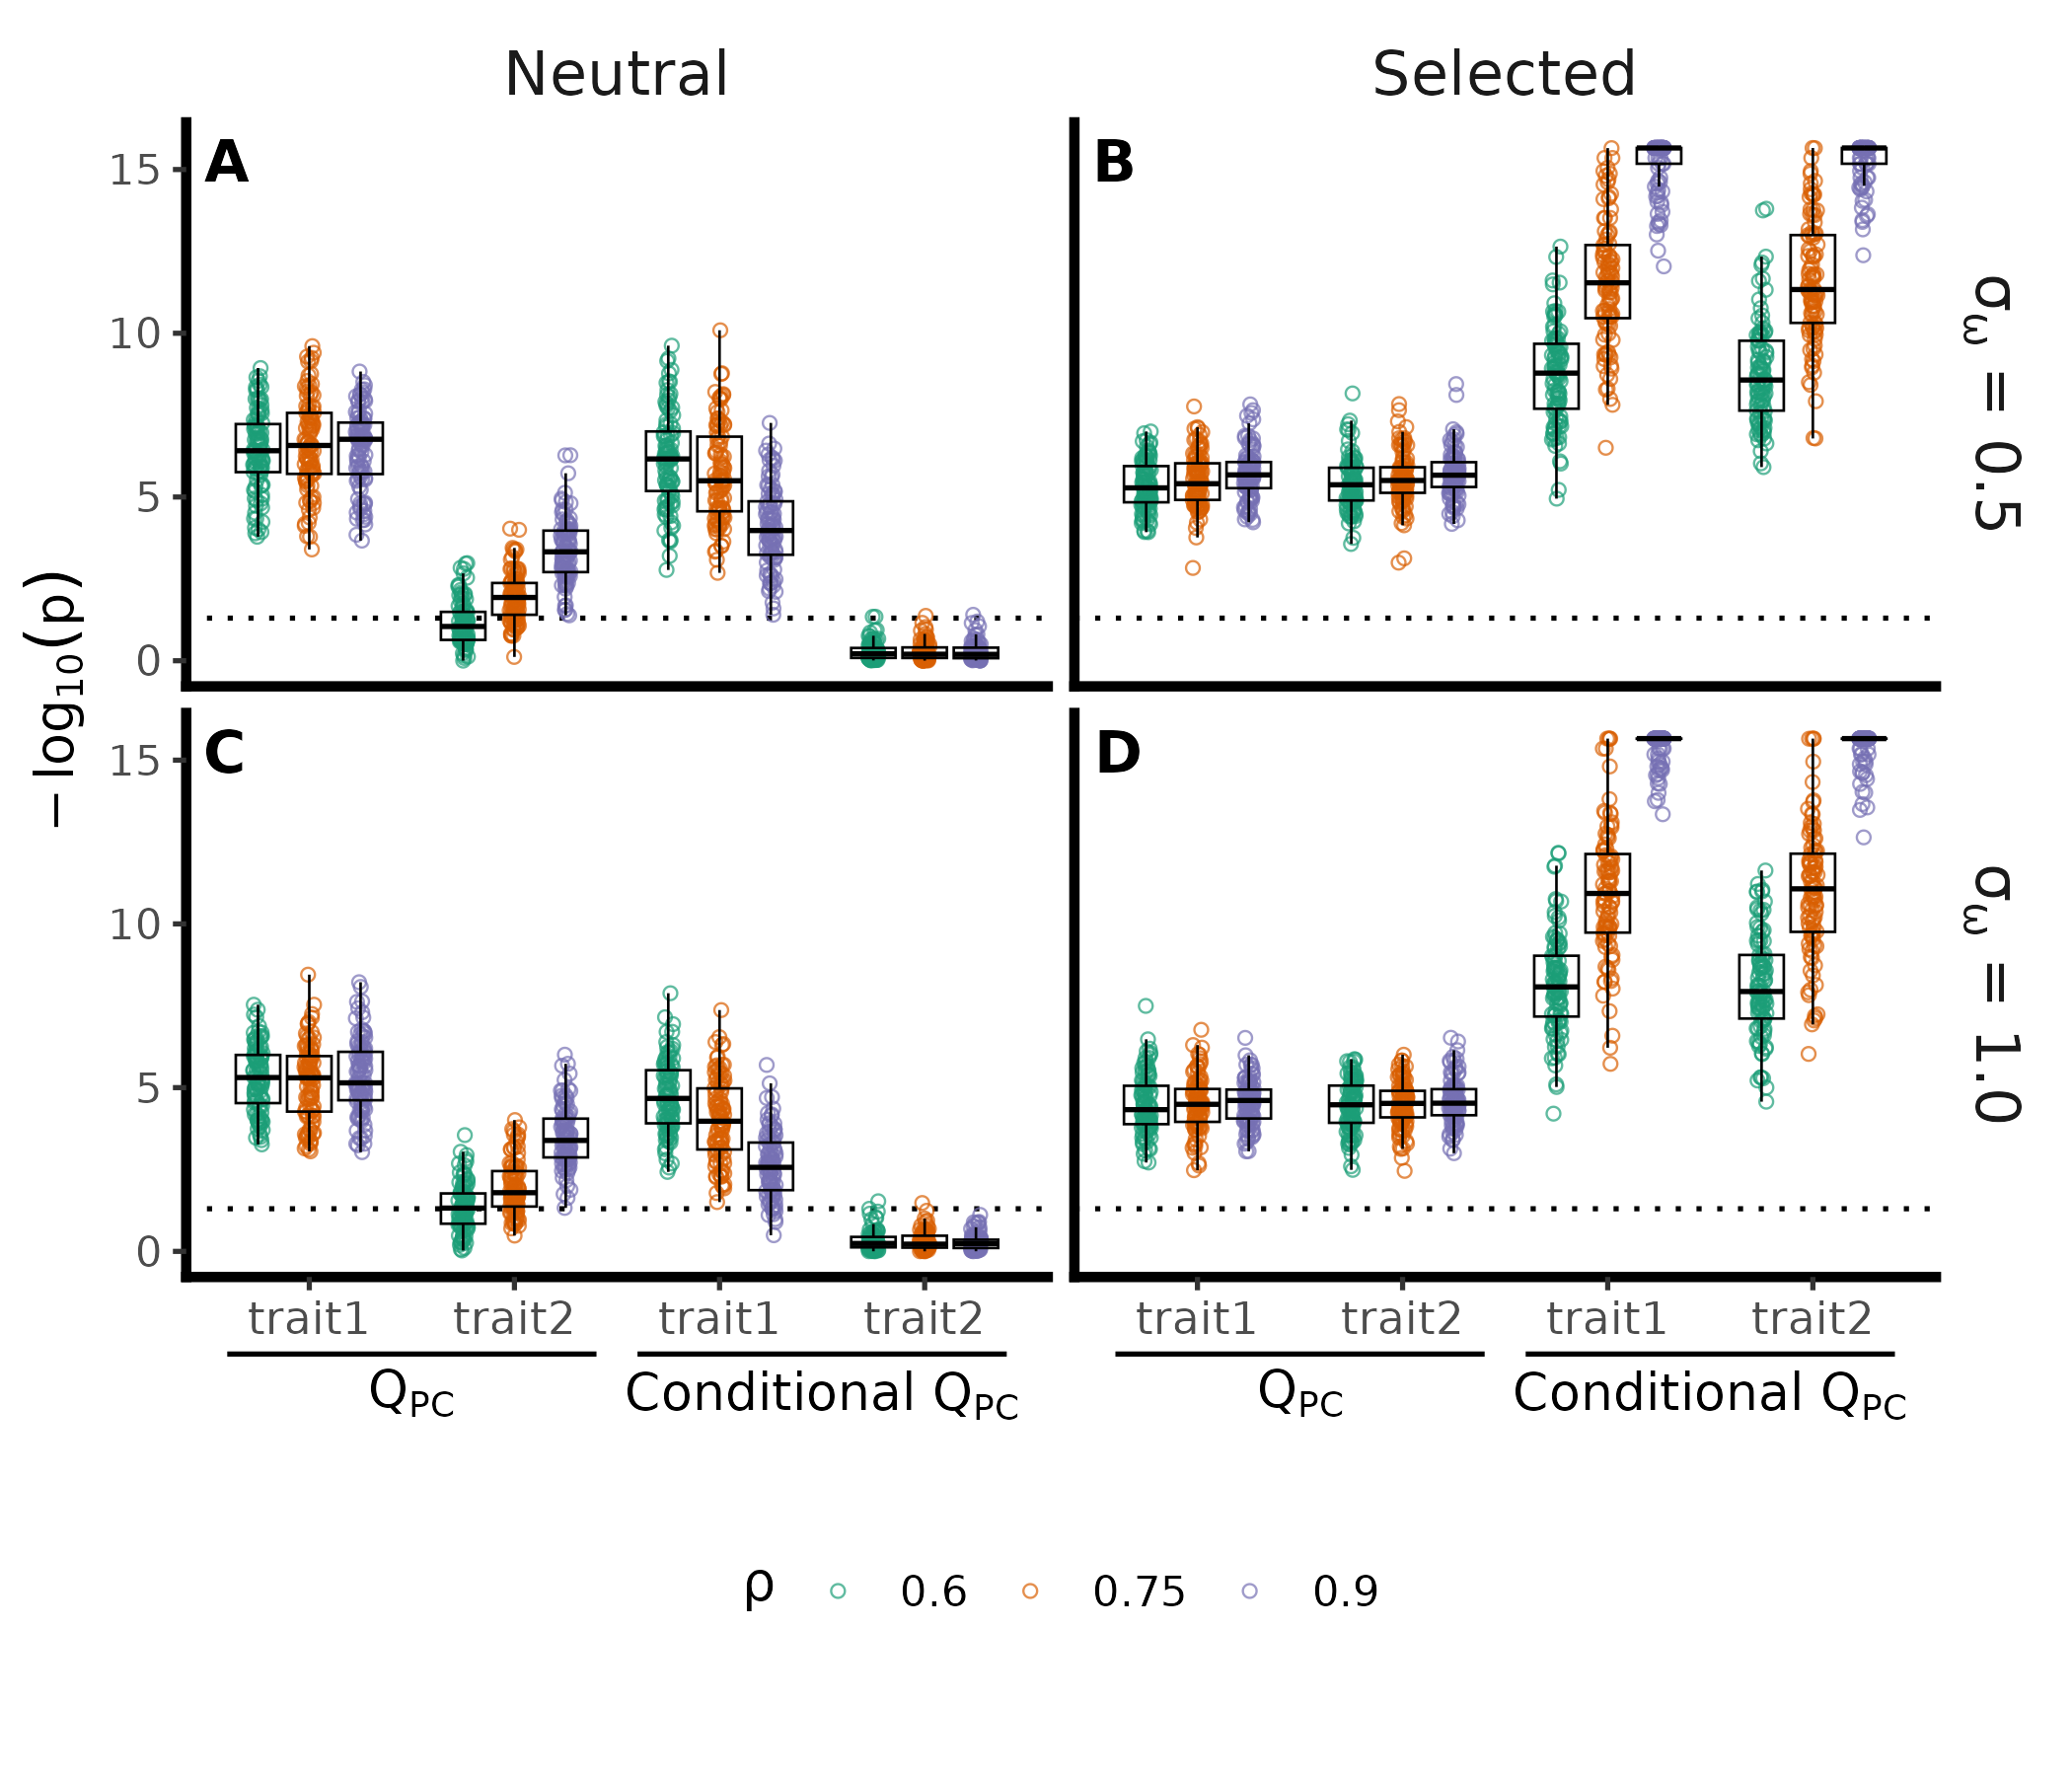
\includegraphics[width=\linewidth]{figures/sim_results_test.png}
\caption{ \textbf{P values from selection tests on simulated traits.}
Results of simulations in SLiM for the four different selection tests run with $-log_{10}(p)$ plotted along the y-axis and the associated test plotted along the x-axis. We simulated trait2 evolving neutrally (A, C) or under selection (B, D) and with condition states under stronger (A, B) or weaker (C, D) selection by varying levels of $\sigma_\omega$. The black dotted line represents a significance threshold of $-log_{10}(0.05) = 1.30$.}
\label{fig:pvalBoxplot}
\end{figure}


\subsection*{Detecting selection on flowering time in individual environments}
We first tested for selection on flowering time within specific environments.
We applied tests for selection on environmental response to a dataset of flowering time measured as days to flowering in 971 \textit{Arabidopsis thaliana} accessions grown in two growth chamber environments: 16 \degree C and 10 \degree C \cite{alonso20161}.
We tested for selection along the first 5 PCs and detected selection along PC 2 for flowering time at 16\degree C (Bonferroni corrected $p = 1.8 \times 10^{-3}$, \ref{fig:ft}A) and selection on flowering time along PC2 at 10\degree C (Bonferroni corrected $p = 0.034$, Fig. \ref{fig:ft}B).
PC2 separates out relict and northern Swedish accessions from the rest of the \textit{A. thaliana} populations.

Flowering time in controlled lab environments may not represent the phenotypic variation that occurs in nature and is under natural selection.
Therefore, we tested for selection on flowering time in 141 accessions planted in two different seasons in the same location in Norwich, England \citep{fournier2011map, wilczek2009effects}.
In the first treatment, 'Fall', seedlings were transplanted into the ground in September and experienced natural cold vernalization while, in the second treatment, 'Spring', seedlings were transplanted into the ground in March and did not experience vernalization. In these experiments, flowering time was measured in photo-thermal units to allow comparisons between different seasonal timepoints.

Using standard $Q_{PC}$ on the first 5 PCs, there was evidence of selection on flowering time in each treatment along PC 3 (Bonferroni corrected $p = 6.06 \times 10^{-3}$, Fig. ~\ref{fig:norwich}A) for Fall and $p = 7.25 x 10^{-4}$ for Spring, Fig. ~\ref{fig:norwich}B).
PC 3 in this population is similar to PC2 in the larger population phenotyped in the lab. Here, PC 3 separates northern Swedish ecotypes from other ecotypes.

 
\subsection*{Detecting selection on reaction norms}
We calculated the difference in flowering time between the  16 \degree C and 10 \degree C environments in the growth chamber and tested for selection on this difference, the reaction norm, along the first five PCs.
We detected evidence for selection on the reaction norm along PC 2 ($p = 0.034$, Fig. \ref{fig:ft}C).
%However, it is unclear how correlations between flowering time in the two environments and the reaction norm affect signatures of selection.
%Flowering time in the two environments and the reaction norm were all correlated with each other (Fig. \ref{fig:ft}D, E).
Flowering time at 16\degree C was significantly correlated with flowering time at 10\degree C (Pearson corr coeff = 0.88) and flowering time at 16\degree C is correlated with the reaction norm (Pearson corr coefficient= 0.82) (Fig. \ref{fig:ft}D, E).
We also calculated a reaction norm for flowering time in the field experiment by taking the difference in flowering time between individuals planted in the fall and in the spring.
The reaction norm showed marginal evidence of selection along PC 3 ($p = 0.0738$, Fig. \ref{fig:fibrRxn}). 

%do we want to do the conditional of rxn norm on the mean?


\begin{figure}[htbp]
  \centering
\includegraphics[width=\linewidth]{figures/floweringtime.eps}
\caption{ \textbf{Testing for selection on flowering time in lab grown \textit{A. thaliana}} Evidence of selection contributing to divergence for flowering time at (A) 16 \degree C, (B) 10\degree C, and (C) the difference between 16 \degree C and 10 \degree C. In all plots, the y axis is measured in days to flower, each dot represents an \textit{A. thaliana} accession, black lines show the linear regression of trait onto PC 2, dashed blue lines show the 95\% confidence intervals for neutral evolution. (D) shows the correlation between flowering time at 16 \degree C and 10\degree C and (E) shows the correlation between flowering time at 16\degree C and the difference in flowering time between the two temperatures. \textcolor{purple}{update to look at corr with the mean across environments}
}
\label{fig:ft}
\end{figure}

\subsection*{Using the conditional test to assess selection independently across environments}

In growth chamber conditions, there was no evidence of selection on the reaction norm of the difference between flowering at 10\degree C and 16\degree C conditional on the mean across environments ($p=0.251$), suggesting that the divergence in the reaction norm among populations could be explained by selection on trait means.
There was also no evidence of selection along PC 3 on the reaction norm in the field-grown plants after conditioning on the mean across environments ($p=0.439$).

Alternatively, we could use the conditional test to test whether selection on a trait in one environment is independent of selection on that trait in a different environment, as expected if divergent selection shapes plasticity.
To assess the independence of selection on flowering time in the two environments, we used the conditional version of $Q_{PC}$ to test for selection on flowering time in each environment conditional on the other, along PC 2.
We found that there was no evidence of selection on flowering time at 10\degree C conditional on flowering time at 16\degree C ($p = 0.244$, Fig. \ref{fig:condft}A), but there was evidence of selection on flowering time at 16 \degree C conditional on flowering time at 10\degree C ($p = 0.00693$, Fig. \ref{fig:condft}B) 
We interpret this as evidence of selection on flowering time at 16 \degree C, and that evidence of selection at 10 \degree C is driven by correlation in flowering time between the two environments.
This result suggests that there is not local adaptation along PC2 for an environmental response to temperature.


To test for evidence of a plastic response to seasonal differences in plants grown in field  conditions, we conducted the conditional test described above, testing for selection in Fall flowering conditional on Spring and vice versa along PC3.
There was evidence of selection on flowering time in vernalized plants conditional on flowering time in unvernalized plants ($p = 0.0123$, Fig. \ref{fig:ellipse}A)) and evidence of selection on unvernalized flowering time conditional on vernalized flowering time ($p = 8.99 \times 10^{-4}$, Fig. \ref{fig:ellipse}B).
We interpret this result as evidence that there has been independent local adaptation on flowering time in two different environments, and this has created genetic variation for plasticity ($G \times E$).

We also visualized patterns of plasticity compared to an expectation based on the G matrix generated from phenotypic variation. 
Eight genotypes from North or South Sweden fell outside the range expected from the joint distribution of phenotypes (Fig. \ref{fig:ellipse}C).
These genotypes all had longer flowering times when planted in the spring than expected based on their fall flowering times, consistent with requiring a strong vernalization to flower.


\begin{figure}[htbp]
  \centering
\includegraphics[width=\linewidth]{figures/conditionaltest.eps}
\caption{ \textbf{Testing for selection on flowering time in \textit{A. thaliana} with the conditional test} The conditional test for selection on flowering time at 10 \degree C conditional on flowering time at 16 \degree C (A) and for flowering time at 16 \degree C conditional on flowering time at 10 \degree C (B). In all plots, each dot represents an \textit{A. thaliana} accession with colors representing population in the same scheme as Fig. \ref{fig:ft}, black lines show the linear regression of trait onto PC 2, dashed blue lines show the 95\% confidence intervals for neutral evolution based on the conditional test. 
}
\label{fig:condft}
\end{figure}

\begin{figure}[htbp]
  \centering
\includegraphics[width=\linewidth]{figures/ellipse.eps}
\caption{ \textbf{The conditional test detects selection on plastic responses to season}. The conditional test for selection on flowering time in Fall plantings conditional on flowering time in Spring plantings (A) and for flowering time in Spring plantings conditional on flowering time in fall plantings (B). In all plots, each dot represents an \textit{A. thaliana} accession with colors representing population, black lines show the linear regression of trait onto PC 2, dashed blue lines show the 95\% confidence intervals for neutral evolution based on the standard test and dashed orange lines show the 90\% confidence intervals for neutral evolution based on the conditional test. Panel C shows the relationship between flowering time in both environemtns and the pink ellipse shows the bounds of the joint $\chi ^2$ distribution of the two phenotypes, corresponding to $\alpha=0.05$ }
\label{fig:ellipse}
\end{figure}



\section*{Discussion}

In this paper, we did \textcolor{pink}{summary goes here}

%Specific for arabidopsis
Previous work in \textit{A. thaliana} has investigated the genetic network contributing to flowering time plasticity\citep{wilczek2009effects}, identified local adaptation \citep{fournier2011map, aagren2013genetic}, and quantified direct selection on flowering time \citep{exposito2018spatio, aagren2017adaptive} and flowering time plasticity in field experiments \citep{fournier2022adaptive}.
In particular, measurements of selection in the field did not detect selection for flowering time plasticity across most sites -- the exception being in one site (Norwich, England) where plants with delayed flowering in the fall planting compared to spring had higher fitness in the spring \citep{fournier2022adaptive}.
This observation matches our results that selection appears to have contributed to divergence in plasticity in response to these environments.

%general relevance of qst-fst approaches and comparison to common garden (Selection on seasonal plasticity was detected only in Norwich spring, where genotypes with high values of PC2 had greater fitness (i.e. genotypes flowering later under short days in fall than under long days in spring and summer).
We may not expect concordance between common garden experiments and \qf.
While common garden experiments can detect selection in a specific year, \qf tests for evidence of selection shaping trait divergence itself.
These tests may provide different answers, especially as global climates more dramatically differ from the climates of past selection.
Recently, \cite{do2025method} developed a method for applying \qf to populations of varying relatedness without relying on principal components. 
It would be interesting to see if the conditional test can be applied to this framework.


%plasticity is confusing paragraph
This approach provides a comprehensive way to test whether selection has shaped between-population divergence in responses to different environments and separate it out from selection on the trait alone. 
This approach is slightly different from testing for evidence of selection on the reaction norm, since the reaction norm is itself a function of trait values within environments. 
However, it may be that for some research questions, the reaction norm approach is more sensible. \emjo{um gotta think of when}


% When will this test be useful
The conditional extension of \qpc could be useful for detecting selection on plasticity across any set of common garden experiments conducted in multiple environments on genotyped individuals.
As more and more diversity panels are developed for genome-wide association mapping, these types of experiments are becoming more common \citep{mead2026variation, MacQueen_2025, fournier2011map}.
However, one limitation of condition \qpc is that it tended to have lower power when traits as measured across environments were highly correlated.
We think that in this case researchers will likely not be motivated to study local adaptation in \gxe since strong correlations across environments necessarily mean that there is either little plasticity or little genetic variation for that plasticity.

An additional limitation of our current implementation of conditional \qpc is that it is limited to testing in two environments.
Many common garden experiments have been conducted across >2 environments, including the \textit{Arabidopsis thaliana} experiment used here.
In the future, expanding the implementation of the conditional test to condition on multiple traits would improve the applicability of the test.
However, it may also strongly reduce power to detect selection.

%Field common garden experiments are very powerful for telling us about fitness and selection on specific traits in a given year.
%But, we know that climates are variable and that trait differentiation is shaped by selection that occurred over many past generations.
%This approach lets us see the effects of that past selection and confirm that flowering time plasticity in the Norwich environment is likely adaptive.

%The relationship between environmental cues and flowering time also likely differ between growth chamber and field environments \citep{bergelson2010towards, Brachi2011, weinig2002novel}.

\section*{Acknowledgments}
Helpful discussions with and/or comments from Graham Coop, Jean-Luc Jannink, Randy Wisser. This work was funded by a National Institutes of Health grant (R35 GM142829) to E.B.J.

\bibliography{mybib}


\beginsupplement

\section*{Supplementary methods}

\subsection*{Testing for selection on reaction norms}
Following the multivariate normal model of drift, the vector of allele frequencies of a single allele across these individuals or populations, under neutrality, is expected to be distributed as follows:
\begin{equation}\label{eq:mvna}
\vec{p} \sim MVN (\epsilon \vec{1}, \epsilon (1-\epsilon) F)
\end{equation}
where $\epsilon$ is the ancestral allele frequency, estimated from the current population mean frequency, and $F$ is the genetic kinship matrix for individuals sampled in $\vec{p}$.

For a quantitative trait whose value is determined by additive combinations of alleles, without dominance or epistasis, we can think of traits as breeding values or polygenic scores where the polygenic score for individual or population $i$ is denoted as $Z_{i}$ and
\begin{equation}\label{eq:pgs}
  z_{i} = 2\sum_{l=1}^{L}\alpha_{l}p_{l},
\end{equation}
where $\alpha_{l}$ is the phenotypic effect size of the non-reference allele at the $l^{th}$ locus, $p_{l}$ is the allele frequency of that locus in that individual or population, and $L$ is the number of loci that effect the trait.
Since the sum of multiple independent normally-distributed variables will also be normally distributed, we can model the neutral distribution of an additive quantitative trait as a multivariate normal (as in Eq. \ref{eq:mvn})


If we  measure plasticity in some way that is based on an additive combination of quantitative traits, like a reaction norm, we will be able to also model this measure of plasticity using a multivariate normal distribution.
To see why, let $\vec{Z_{R}}$ be a vector of reaction norms for a group of $n$ individuals or populations so that if $\vec{Z_{1}}$ and $\vec{Z_{2}}$ are measurements of a trait in two different environments, $\vec{Z_{R}} = \vec{Z_{1}} - \vec{Z_{2}}$.
If $z_{R,i }$ is the value of the reaction norm for a given individual or population $i$, then we can rewrite Eq. \ref{eq:pgs} for $Z_{R}$ in terms of the allelic effects of loci on traits in environments $1$ and $2$ ($\alpha_{l,1}$ and $\alpha_{l,2}$ respectively),
\begin{equation}
z_{R,i} = 2\sum^{L}_{l=1}(\alpha_{l,1}-\alpha_{l,2})p_{l}.
  \end{equation}

The distribution of $\vec{Z_{R}}$ under drift is now
\begin{equation}
\vec{Z_{R}} \sim MVN(\mu_{1} - \mu_{2}, 2(V_{A,1} + V_{A,2} - 2C_{A, 12})),
\end{equation}
where $\mu_{1}$ is the mean of trait1, $\mu_{2}$ is the mean of trait2, $V_{A,1}$ is the additive genetic variation for trait1, $V_{A,2}$ is the additive genetic variation for trait2, and $C_{A,12}$ is the covariance of the two traits.
Crucially, $Z_{R}$ still follows a multivariate normal distribution and can be related back to the multivariate normal expectation for allele frequencies in Eq. \ref{eq:mvna}.

We might also be interested in testing for selection on measures of plasticity that are not made up of linear combinations of trait measurements made across environments.
For example, some researchers measure plasticity using the coefficient of variation or the mean squared error from a reaction norm \citep{scheepens2018phenotypic, catlin2025structural}.

However, we cannot model these non-linear measures of plasticity with the multivariate normal distribution.
To explain why, we describe an example based the variance for trait measurements ($z_{v}$) made in two different environments, where $z_{1,i}$ is individual $i$'s trait in environment $1$ and $z_{2,i}$ is that individual's trait in environment $2$.
Individuals whose trait expression is more sensitive to environment will have higher values of $z_{v}$ than individuals that are less sensitive to the environment.
For an individual $i$,
\begin{equation}
  z_{v,i} = \textbf{E}([z_{1,i}^{2}, z_{2,i}^{2}]) - \textbf{E}([z_{1,i}, z_{2,i}])^{2}
  %= \frac{1}{4}(z_{1,i}^{2} +z_{2,i}^{2}) - [\frac{1}{2}(z_{1,i}+z_{2,i})]^{2}
 % = \frac{1}{4}(z_{1,i}^2 + z_{2,i}^2)-\frac{1}{2}z_{1,i}z_{2,i}
 =\frac{1}{4}(z_{1,i} - z_{2,i})^2
    \end{equation}

Since the values $z_{1,i}$ and $z_{2,i}$ can be written in terms of the allele frequencies of the $L$ loci and the allelic effects of these loci on trait in environment 1 ($\alpha_{1}$) and environment 2 ($\alpha_{2}$), the variance measure of plasticity $z_{v,i}$ can also be written in terms of allele frequencies and effect sizes.
\begin{equation}\label{eq:zvi}
z_{v,i} = 
%\frac{1}{4}\sum^{L}_{l=1}[2(\alpha_{1,l}^{2} + \alpha_{2,l}^{2})p_{l,i}^{2} - 2(\alpha_{1,l} + \alpha_{2,l})p_{l,i}]\\
\frac{1}{2}[\sum^{L}_{l=1}(\alpha_{1,l}-\alpha_{2,l})p_{l,i}]^2
  \end{equation}

Crucially, Eq. \ref{eq:zvi} shows that since $z_{v,i}$ cannot be written in terms of additive combinations of allele frequencies and allelic effects.
Therefore, even though the allele frequencies of the loci that affect the trait can be modeled following the multivariate normal distribution, we cannot model $z_{v}$ as a multivariate normal distribution.


\subsection*{Conditional tests for adaptive differentiation}
As an alternative to detecting selection on reaction norms, we adapted $Q_{PC}$ to test for excess trait differentiation in a focal trait conditional on differentiation in a second trait.
We base our use of the conditional test on \cite{Berg2017}, who developed a two-trait conditional test for polygenic adaptation.
We discuss two traits here, but we intend to use these analyses in situations where the two traits are measurements of the same trait in two different environments.

We first extend the model for a neutral distribution of a trait to deal with two correlated traits.
If $\vec{Z_{1}}$ is a vector of trait values for a set of individuals and $\vec{Z_{2}}$ is a vector of trait values for a different trait in those same individuals, we can model the joint distribution of these trait values under neutrality as follows

\begin{equation}\label{eqn:mvn2trait}
  \begin{bmatrix}
\vec{Z_{1}} \\ \vec{Z_{2}}
  \end{bmatrix} \sim MVN\bigg(
  \begin{bmatrix}  \mu_{1}\vec{1}\\ \mu_{2}\vec{1} \end{bmatrix}, 2
   \begin{bmatrix} V_{A,1}F & C_{A,12}F\\ C_{A, 12}F & V_{A,2}F
    \end{bmatrix}\bigg),
\end{equation}

where $\mu_{1}$ is the mean of $\vec{Z_{1}}$, $\mu_{2}$ is the mean of $\vec{Z_{2}}$, $F$ is the kinship matrix of individuals, $V_{A,1}$ is the additive genetic variance of trait1, $V_{A,2}$ is the additive genetic variance of trait2, and $C_{A,12}$ is the additive genetic covariance of traits 1 and 2.

Following Eq. \ref{eqn:mvn2trait}, we can model the neutral distribution of trait1 conditional on the distribution of trait2.
\begin{equation}\label{eq:cond}
\vec{Z_{1}}|\vec{Z_{2}} \sim MVN(\vec{\mu'}, 2V_{A,1}'F)
\end{equation}
where $\vec{\mu'}  = \mu_{1} + \frac{C_{A,12}}{V_{A,2}}(\vec{Z_{2}} - \mu_{2}) $ is a vector of conditional means and $V_{A,1}' =  V_{A,1} - \frac{C_{A,12}^{2}}{V_{A, 2}}$ is the conditional additive genetic variance of trait1.

Following \cite{Josephs2019}, we project the traits $Z_{1}$ and $Z_{2}$ onto the genetic PCs of our samples, which we determine by calculating the eigenvectors of the kinship matrix $F$.
We define the standardized projection of trait $X_{1}$ onto the $m^{th}$ PC as $X_{1m}$, so that if $\vec{U_m}$ is the eigenvector of the $m^{th}$ PC and $\lambda_{m}$ is the corresponding eigenvalue,
\begin{equation}\label{eq:proj}
X_{1,m} = \frac{(\vec{Z_{1}}-\vec{\mu_{1}})\vec{U_{m}}}{\sqrt{\lambda_{m}}}
  \end{equation}
Using the affine transform of equation \ref{eq:mvn} (as shown in \cite{Josephs2019}), $X_{1,m} \sim N(0, 2V_{A1})$ and we can estimate $V_{A,1}$ and $V_{A,2}$ from a subset of $\mathbb{L}$ PCS following Eq \ref{eq:vaest} and $C_{A,12}$ following similar logic. 

%We then estimate trait variances and covariances as follows:
%\begin{equation}
%V_{A,1} = \textnormal{Var}(X_{1,L}) = \textbf{E}[X_{1,L}^{2}],
%  \end{equation}
%\begin{equation}
%V_{A,2} = \textnormal{Var}(X_{2,L}) = \textbf{E}[X_{2,L}^{2}],
%\end{equation}
%and
%\begin{equation}
%C_{A,12} = \textnormal{Cov}(X_{1,L}, X_{2,L}) = %\textbf{E}[X_{1,L}X_{2,L}].
%\end{equation}
We can then test for evidence of selection on $Z_{1}$ conditional on $Z_{2}$ by combining equations \ref{eq:proj} and \ref{eq:cond} to get an expected distribution of the difference between observed values and conditional means projected onto a PC $m$ that is not contained within the subset $L$ used to estimate genetic variances and covariances:
\begin{equation}
\frac{(Z_{1} - \vec{\mu_{1}'})\vec{U_{m}}}{\sqrt{2V_{A,1}'\lambda_{m}}} = X_{m, cond} \sim N(0,1)
  \end{equation}
Seeing a value of $X_{m,cond}$ that falls outside the normal distribution is consistent with selection. 



%\subsection{Conditional test on reaction norms}
%The conditional test could provide a way to test for evidence of selection on a reaction norm while removing selection on the trait itself.
%For example, we can generate a conditional expectation for the reaction norm based on trait expression in a single environment.
%\begin{equation}
%\vec{Z_{R}}|\vec{Z_{1}} \sim MVN(\vec{\mu_{R}'}, V_{A,R}'F)
%\end{equation}
%where
%\begin{equation}
%  \vec{\mu_{R}'}  = \mu_{R} + \frac{C_{A,1R}}{V_{A,1}}(\vec{Z_{1}} - \mu_{1}) = \mu{_1} - \mu_{2} + \frac{V_{A,1} - C_{A, 12}}{V_{A,1}}(\vec{Z_{1}} - \mu_{1})
%\end{equation}
%and
%\begin{equation}
%  V_{A,R}' =  V_{A,R} - \frac{C_{A,1R}^{2}}{V_{A, 1}} = V_{A,1}V_{A,2} - C_{A,12} - \frac{(V_{A,1} - C_{A,12})^{2}}{V_{A,1}}.
%  \end{equation}

\begin{figure}[htbp]
  \centering
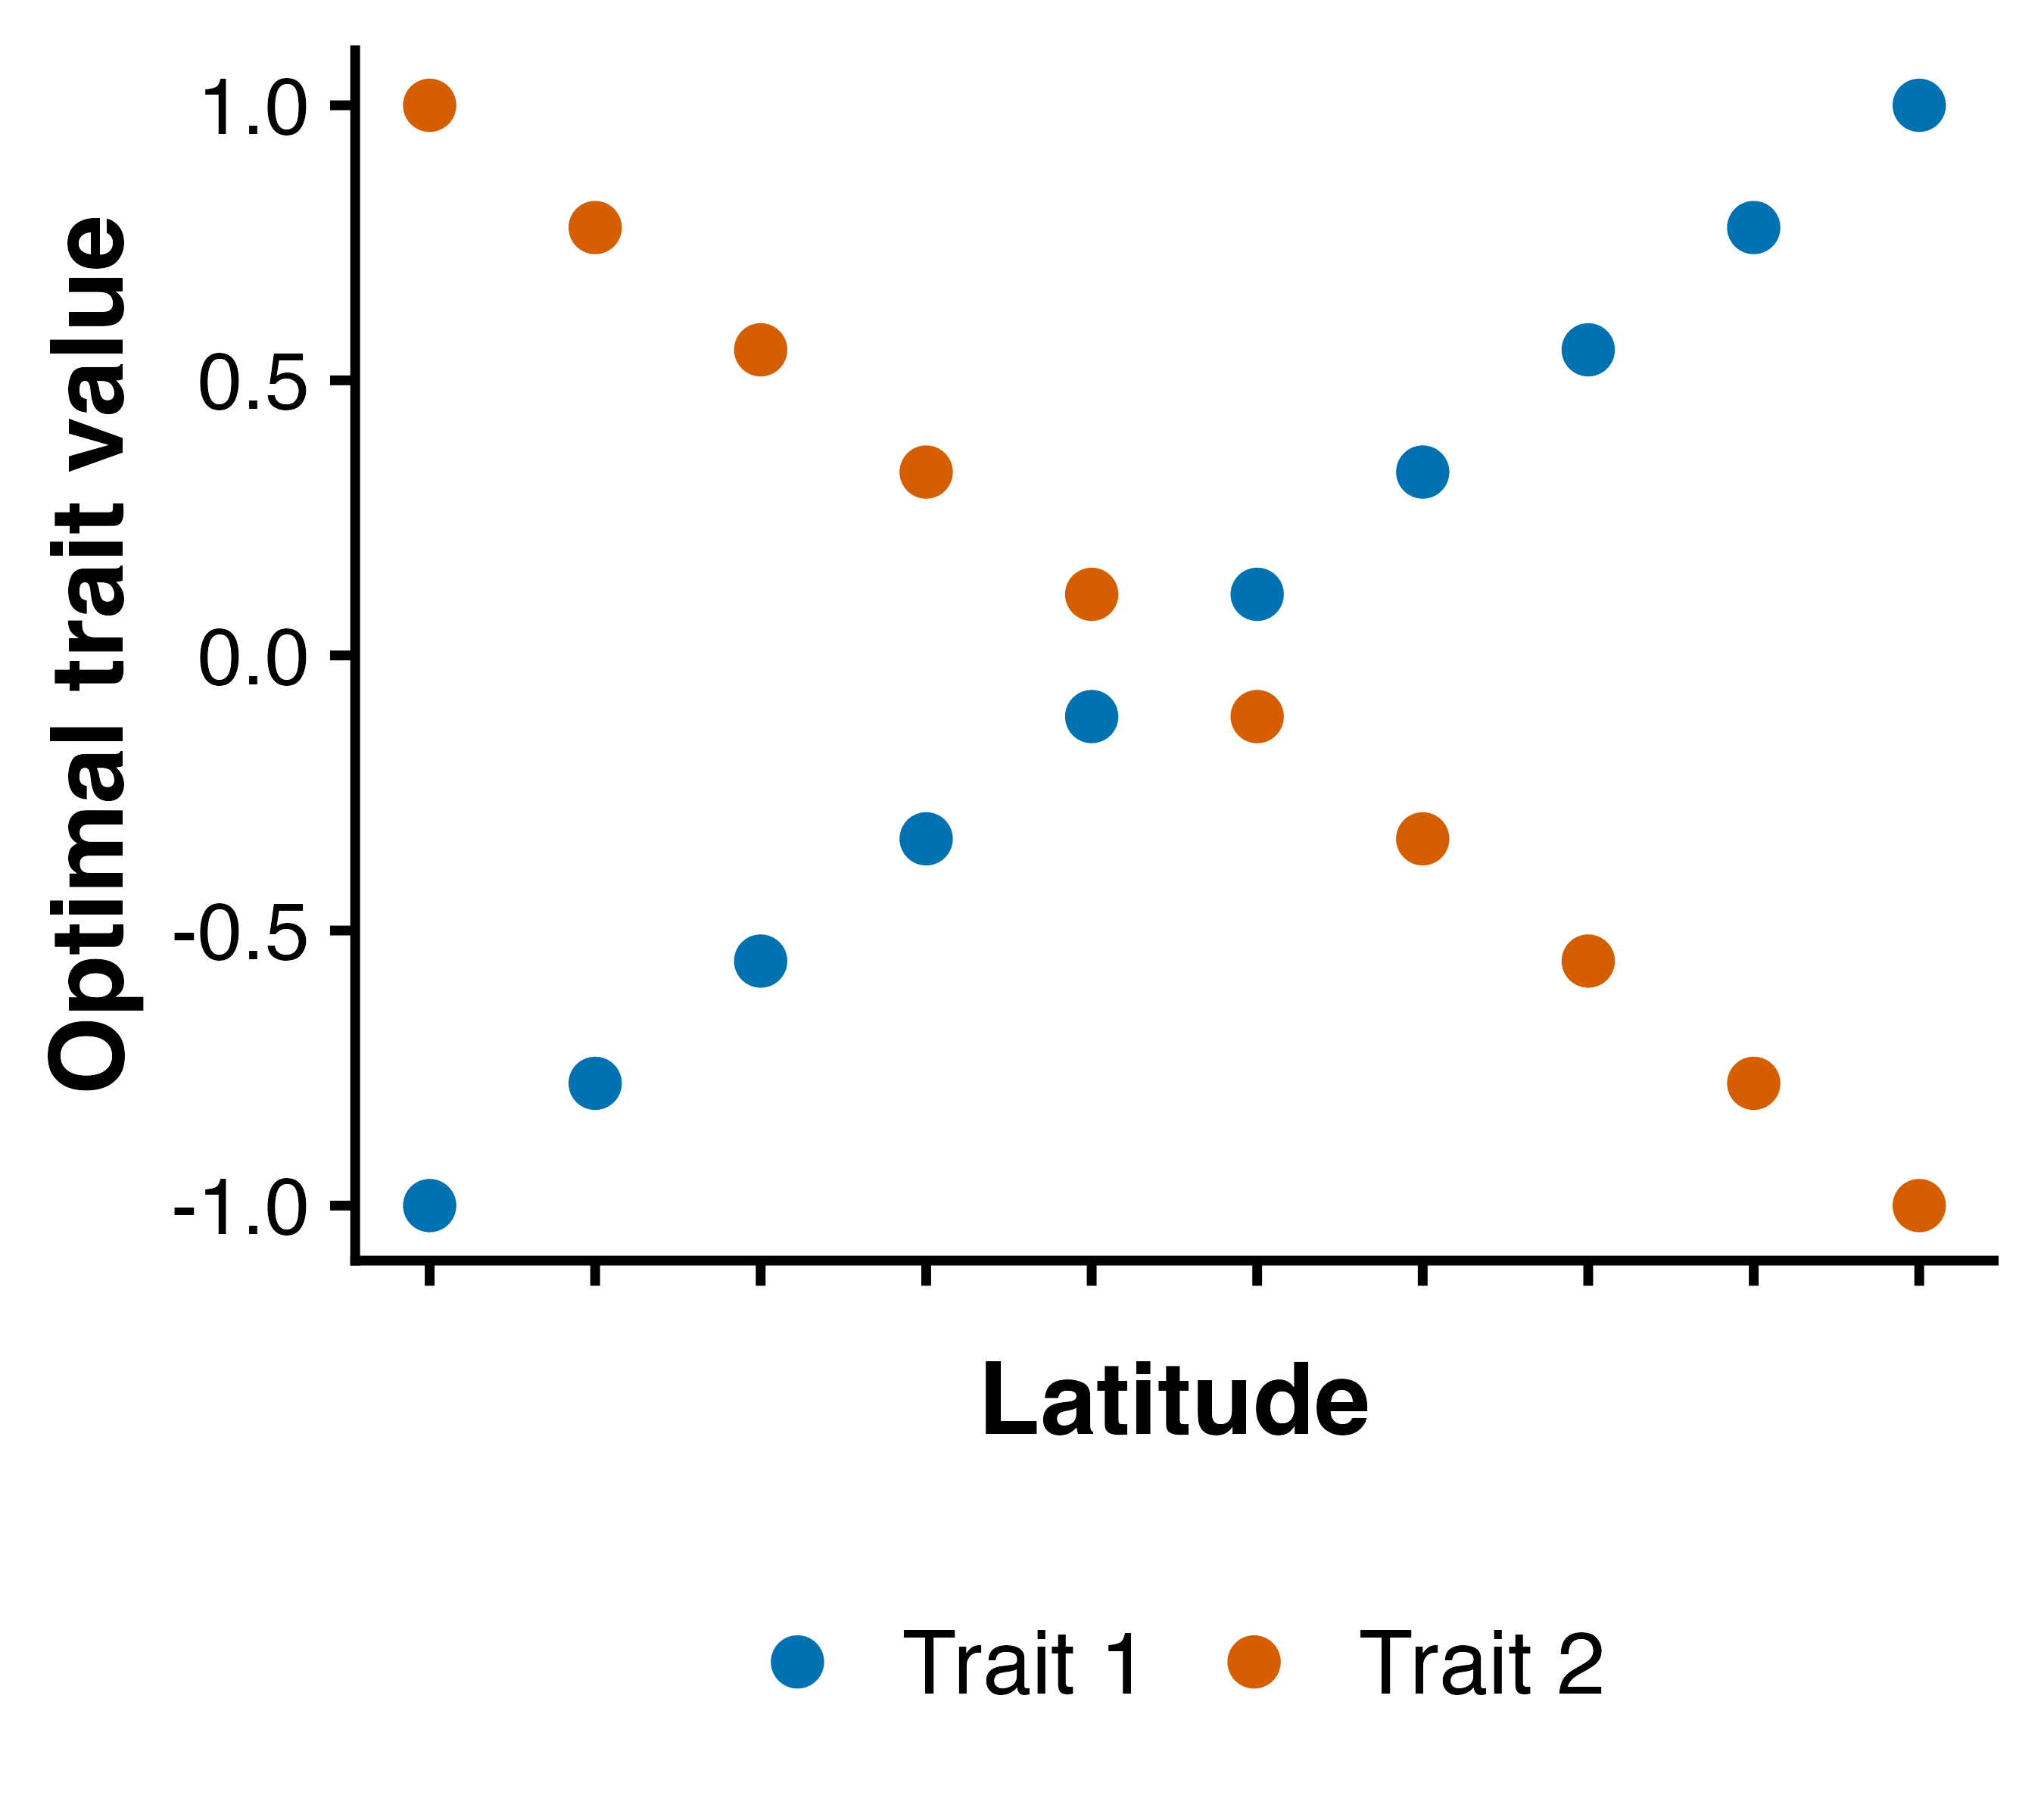
\includegraphics[width=\linewidth]{figures/optimal_trait_values.png}
\caption{\textbf{Final optimal trait values for SLiM simulations.} Optimal trait values for trait1 (blue) and trait2 (orange) at each latitude after the initial burn-in for the SLiM simulations. The optima changed from $0.0$ during burn-in to their final values in a stepwise fashion over 5000 generations. }
\label{fig:simOptima}
\end{figure}


\begin{figure}[htbp]
  \centering
\includegraphics[width=\linewidth]{figures/FIBRnorwich.eps}
\caption{\textbf{Testing for selection on wild grown plants.}  Evidence of selection on flowering time in \textit{A. thaliana} planted in the Spring (A) and Fall(B). In all plots, each dot represents an \textit{A. thaliana} accession with colors representing population in the same scheme as Fig. \ref{fig:ft}, black lines show the linear regression of trait onto PC 2, dashed blue lines show the 95\% confidence intervals for neutral evolution based on the conditional test. }
\label{fig:norwich}
\end{figure}


\begin{figure}[htbp]
  \centering
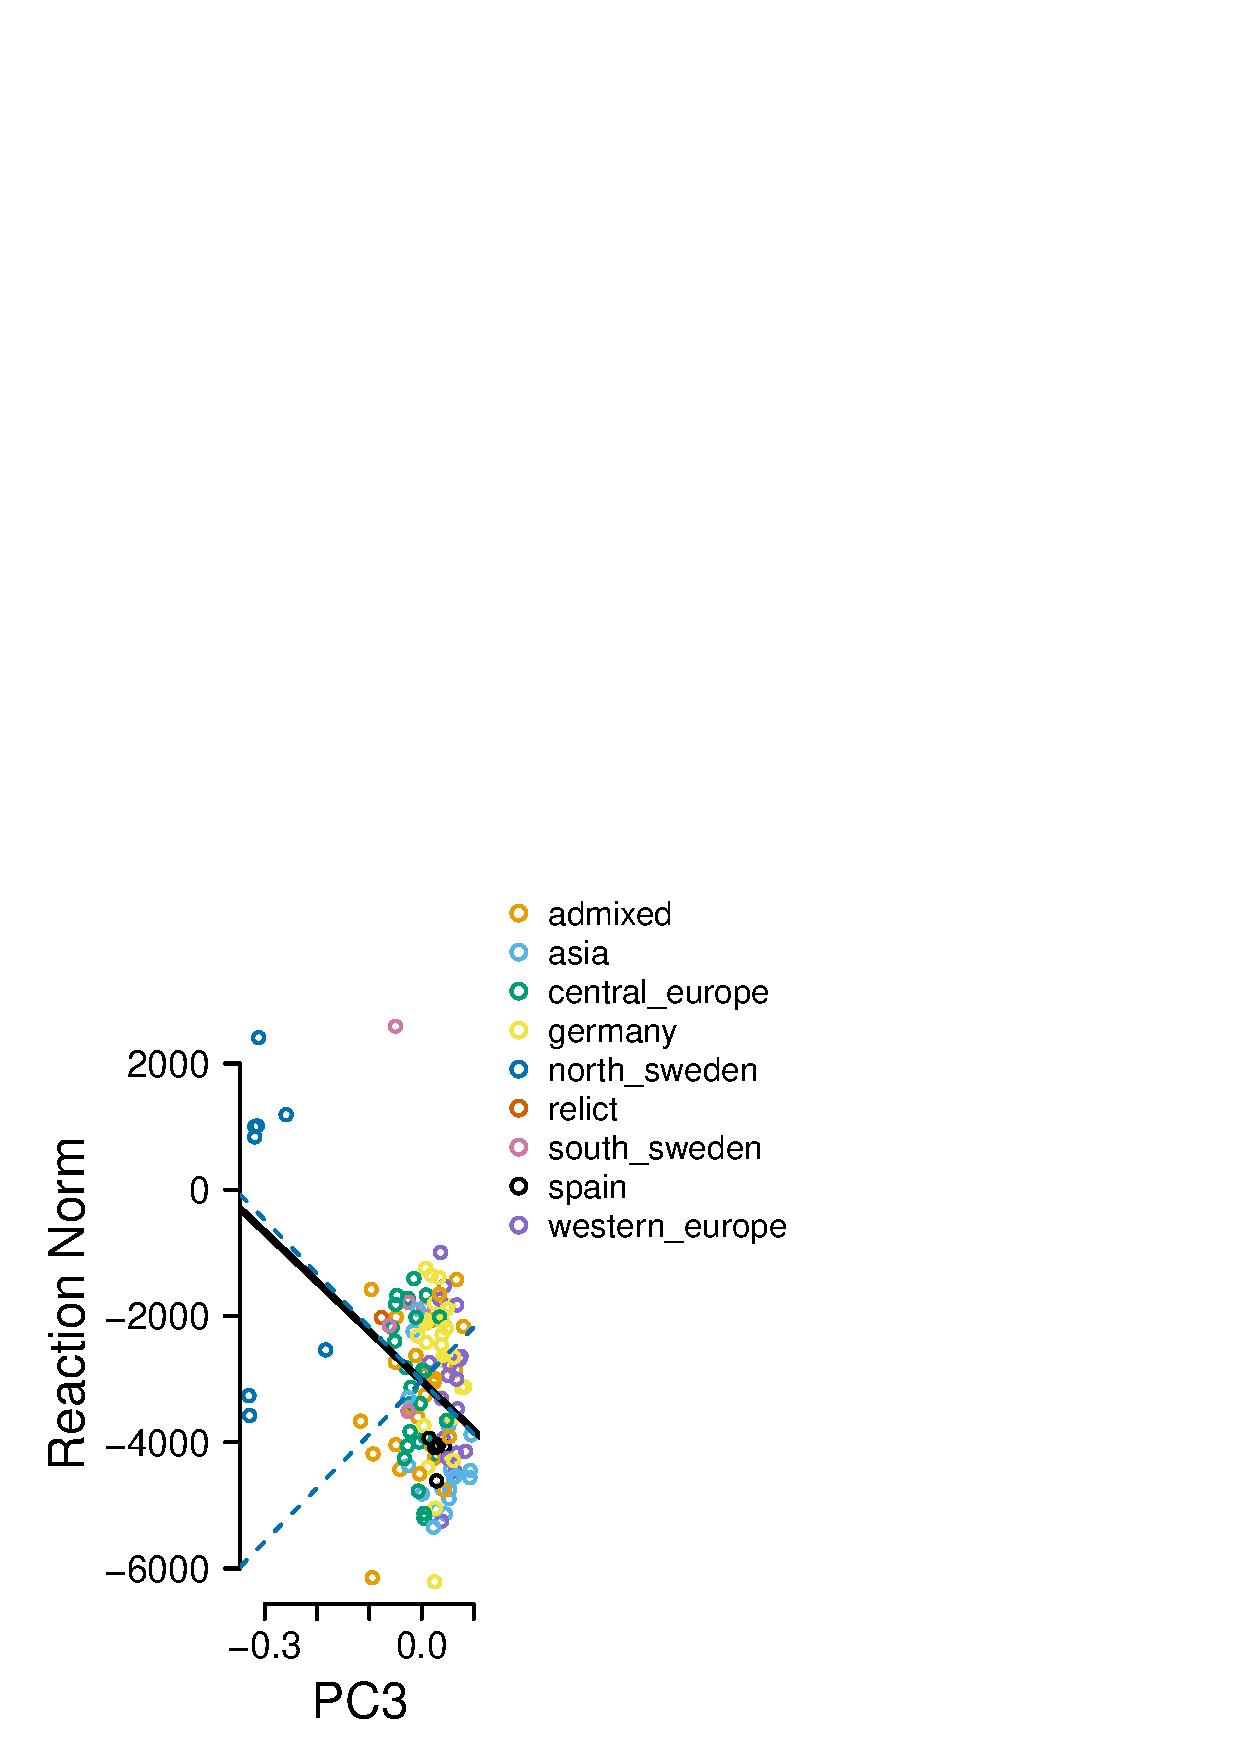
\includegraphics[width=\linewidth]{figures/FIBRnorwichRxn}
\caption{\textbf{Testing for selection on flowering time reaction norm.} The reaction norm of PTUs to bolt for individuals planted in the fall and in the spring. In all plots, each dot represents an \textit{A. thaliana} accession with colors representing population in the same scheme as Fig. \ref{fig:ft}, black lines show the linear regression of trait onto PC 2, dashed blue lines show the 95\% confidence intervals for neutral evolution based on the conditional test.}
\label{fig:fibrRxn}
\end{figure}


\end{document}
